%! TeX program = lualatex
\documentclass[../main.tex]{subfiles}
\begin{document} \section{Continuous random variables}

A random variable is a continuous random variable if it takes values on an interval.  Continuous random variables are described by their PDF or CDF which we introduce below. 

\begin{definition}[probability density function (PDF)]
  The \hlmain{probability density function} for a \emph{continuous} random variable \(X\) is a non-negative continuous function \(f(x)\) that satisfies
  \[
    \mathbb{P}(a \le X \le b) \phantom{ = \int_{a}^{b} f(x) \;dx.} \hspace{1in}
  \]
\end{definition}
\blanklines{10}

\faStar{} If \(X\) is a continuous random variable, then \(\mathbb{P}(X = c) = \underline{\hspace{1cm}}\) for any constant \(c\).
\blanklines{5}

\faStar{} A valid PDF \(f_{X}\) must satisfy \(\int_{-\infty}^{\infty} f(x) \;dx = \underline{\hspace{1cm}}\). 
\blanklines{5}

\begin{example}
  Which of the followings are valid PDFs?

  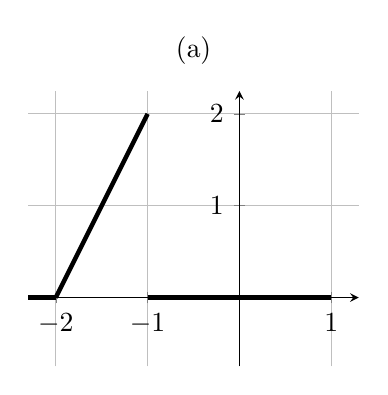
\begin{tikzpicture}
    \begin{axis}[xmin={-2}, xmax={1}, ymin={-0.5}, ymax={2}, title={(a)}, height={2in}, no markers, grid=major, axis lines=middle, enlargelimits, axis equal image, ytick={0,1,2}]
      \addplot[ultra thick] coordinates { (-3,0) (-2,0) };
      \addplot[ultra thick] coordinates { (-2,0) (-1,2) };
      \addplot[ultra thick] coordinates { (-1,0)  (1,0) };
    \end{axis}
  \end{tikzpicture}
  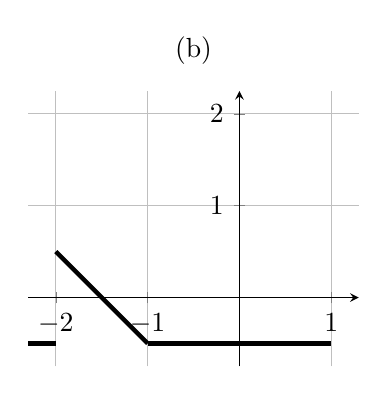
\begin{tikzpicture}
    \begin{axis}[xmin={-2}, xmax={1}, ymin={-0.5}, ymax={2}, title={(b)}, height={2in}, no markers, grid=major, axis lines=middle, enlargelimits, axis equal image, ytick={0,1,2}]
      \addplot[ultra thick] coordinates { (-3,-0.5) (-2,-0.5) };
      \addplot[ultra thick] coordinates { (-2, 0.5) (-1,-0.5) };
      \addplot[ultra thick] coordinates { (-1,-0.5) ( 1,-0.5) };
    \end{axis}
  \end{tikzpicture}
  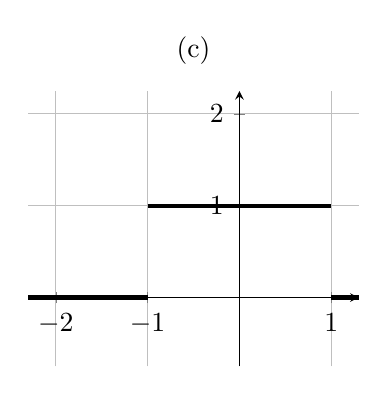
\begin{tikzpicture}
    \begin{axis}[xmin={-2}, xmax={1}, ymin={-0.5}, ymax={2}, title={(c)}, height={2in}, no markers, grid=major, axis lines=middle, enlargelimits, axis equal image, ytick={0,1,2}]
      \addplot[ultra thick] coordinates { (-3,0) (-1,0) };
      \addplot[ultra thick] coordinates { (-1,1) (1,1) };
      \addplot[ultra thick] coordinates { (1,0) (2,0) };
    \end{axis}
  \end{tikzpicture}
  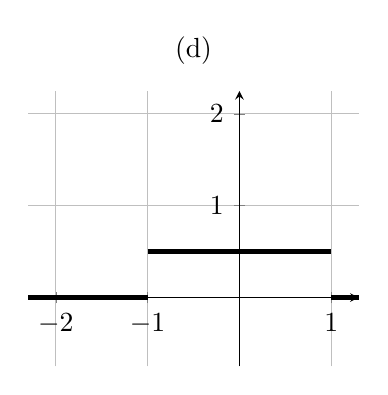
\begin{tikzpicture}
    \begin{axis}[xmin={-2}, xmax={1}, ymin={-0.5}, ymax={2}, title={(d)}, height={2in}, no markers, grid=major, axis lines=middle, enlargelimits, axis equal image, ytick={0,1,2}]
      \addplot[ultra thick] coordinates { (-3,0) (-1,0) };
      \addplot[ultra thick] coordinates { (-1,1/2) (1,1/2) };
      \addplot[ultra thick] coordinates { (1,0) (2,0) };
    \end{axis}
  \end{tikzpicture}
\end{example}
\clearpage

Let's pick up some confidence for calculations.  Many PDFs are described as piecewise functions.
\begin{example}
  Suppose \(a\) is a positive constant. Calculate \(\mathbb{P}( 0 \le X \le a/3 )\) given that a continuous random variable \(X\) is described by the PDF
  \[
    f(x) = 
    \begin{cases}
      \frac{1}{2a} & \text{if } -a \le x \le a \\
      0 & \text{otherwise}
    \end{cases}.
  \]

  % Calculate the expectation and variance of \(X\).
  \blanklines{5}
\end{example}

\begin{example}
  Calculate \(\mathbb{P}(-1 < X < 3)\) given that a continuous random variable \(X\) is described by the PDF
  \[
    f(x) = 
    \begin{cases}
      \frac{x^{2}}{3}, & \text{if } 1 \le x \le 2 \\
      1/9, & \text{if } -5 \le x \le -3 \\
      0, &\text{otherwise}
    \end{cases}.
  \]

  \blanklines{10}
\end{example}

We often (in reality and in this course) need to find a suitable PDF for a continuous random variable that suit our needs.  The idea is to set up an equation involving the unknown parameter using the given information and solve for the unknown. Also see Example~\ref{ex:uniform-distribution-from-mean-and-stddev} for a preview.
\begin{example} \label{ex:distribution-with-unknown-bounds}
  The PDF for a continuous random variable is given by \(f(x) = a x^{2}\) if \(|x| < a\) and \(f(x) = 0\) everywhere else.  Find the unknown parameter \(a\).

  \blanklines{15}
\end{example}
\clearpage

Like discrete random variables, a continuous random variable can be described by a CDF, and we can convert between PDF and CDF. 

\begin{definition}[cumulative distribution function (CDF)]
  A function \(F(x)\) is a \hlmain{cumulative distribution function} for a continuous random variable \(X\) if
  \[
    \mathbb{P}(X \le x) \hspace{2in}
  \]
\end{definition}

\faStar{} A valid CDF must be non-decreasing and satisfy \(\lim_{x \to -\infty} F(x) = 0\) and \(\lim_{x \to \infty} F(x) = 1\).

\begin{center}
  \begin{tikzpicture}
    \begin{axis}[title={CDF}, smooth, samples=100, width=5in, height=2in, axis lines=middle, enlargelimits, xmin=-2, xmax=2, ymin=0, ymax=1, ytick={0.5, 1}, yticklabels={,1}, xtick={-2,-1,0,1,2}]
      \addplot[very thick, domain=-2:2] {1/(1 + exp(-0.07056*x^3 - 1.5976*x))};
      \addplot[dashed] coordinates {(-3,1) (3,1)};
      \addplot+[main, mark=*, mark options={fill=main}] coordinates {(-0.3, 0.381972)};
    \end{axis}
  \end{tikzpicture}

  \begin{tikzpicture}
    \begin{axis}[title={PDF}, smooth, samples=100, width=5in, height=2in, axis lines=middle, enlargelimits, ymin=0, ymax=1, ytick={0.5, 1}, yticklabels={,1}, xtick={-2,-1,0,1,2}]
      \addplot[domain=-2:-0.3, name path=f] {e^(-x^2)/sqrt(2*pi)};
      \addplot[domain=-2:-0.3, name path=g] {0};
      \addplot[fill=main!50] fill between [of=f and g];
      \addplot[very thick, domain=-2:2] {e^(-x^2)/sqrt(2*pi)};
      
    \end{axis}
  \end{tikzpicture}
\end{center}

\faStar{} If the PDF for a random variable \(X\) is known, then it is very easy to find its CDF. 
\blanklines{5}

\faStar{} Conversely, if the CDF for a continuous random variable \(X\) is known, then it is only one differentiation away from getting the PDF of \(X\).
\blanklines{5}

\clearpage

\begin{example}
  Calculate \(\mathbb{P}(-0.5 \le X \le 0.3)\) given that the CDF for a continuous random variable \(X\) is 
  \[
    F(x) = 
    \begin{cases}
      0 & \text{if } x < -1 \\
      \frac{x + 1}{2} & \text{if } -1 \le x \le 1 \\
      1 & \text{if } x > 1
    \end{cases}.
  \]
  Moreover, find its PDF.
  \blanklines{10}
\end{example}

\begin{example}[a normal distribution]
  The PDF for a continuous random variable \(X\) is \[f(x) = \frac{1}{\sqrt{2 \pi}} e^{-x^{2}}.\] Express its CDF as an integral. 

  \blanklines{5}
\end{example}
\end{document}
